
\section{Functional Requirements}

% Content goes here
\subsection{User Authentication}
The system shall provide user authentication functionality to ensure that only authorized users can access the system. This functionality should include the following requirements:

\begin{itemize}
    \item The system shall allow users to create an account by providing a unique username and password.
    \item The system shall store user credentials securely to protect against unauthorized access.
    \item The system shall provide a login page where users can enter their credentials to access the system.
    \item The system shall enforce password complexity rules, such as minimum length and the use of alphanumeric characters.
    \item The system shall support password recovery options, such as email verification or security questions.
\end{itemize}

\subsection{Data Management}
The system shall provide functionality for managing data. This functionality should include the following requirements:

\begin{itemize}
    \item The system shall allow users to create, read, update, and delete data records.
    \item The system shall enforce data validation rules to ensure the integrity and consistency of the data.
    \item The system shall provide search and filtering capabilities to allow users to find specific data records.
    \item The system shall support data import and export functionality to facilitate data exchange with other systems.
\end{itemize}

\subsection{Reporting}
The system shall provide reporting functionality to allow users to generate and view reports based on the stored data. This functionality should include the following requirements:

\begin{itemize}
    \item The system shall provide predefined report templates for common use cases.
    \item The system shall allow users to customize report templates or create new ones.
    \item The system shall support exporting reports in various formats, such as PDF or Excel.
    \item The system shall provide options for scheduling and automating report generation.
\end{itemize}

% Optional placeholders for figures
\begin{figure}[ht]
    \centering
    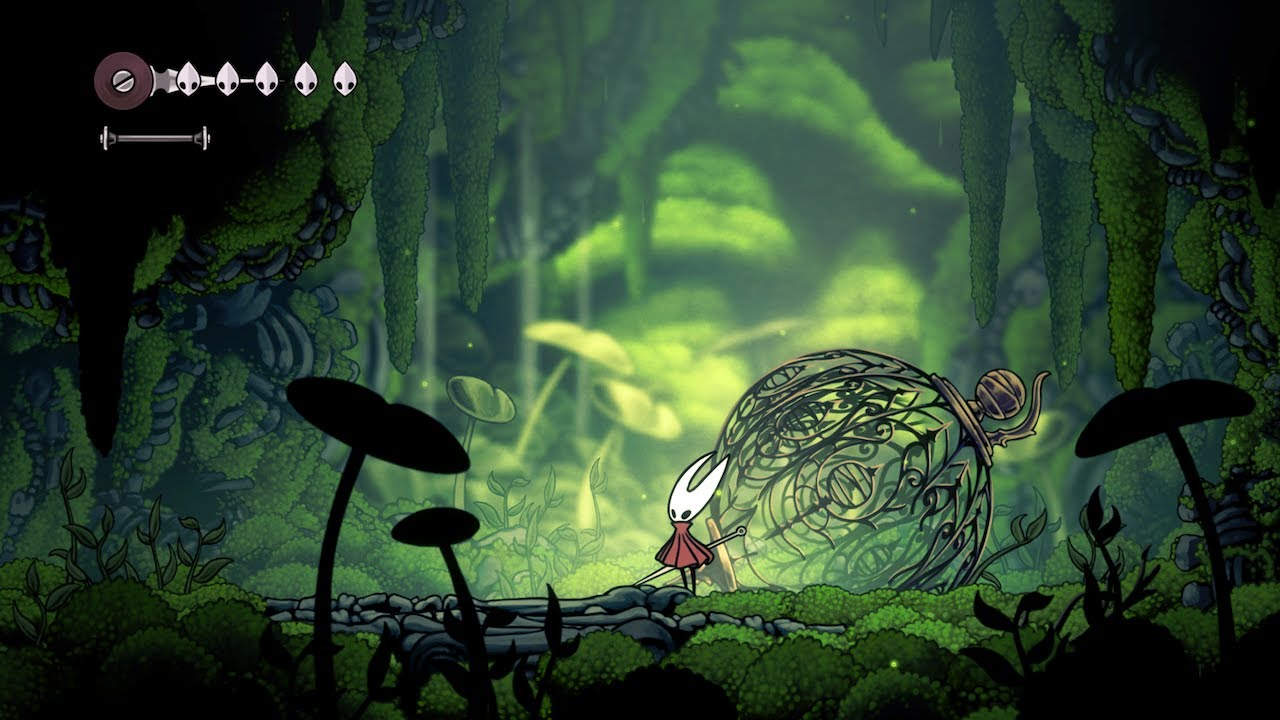
\includegraphics[width=0.8\textwidth]{images/figure1}
    \caption{Example figure 1}
    \label{fig:figure1}
\end{figure}

\begin{figure}[ht]
    \centering
    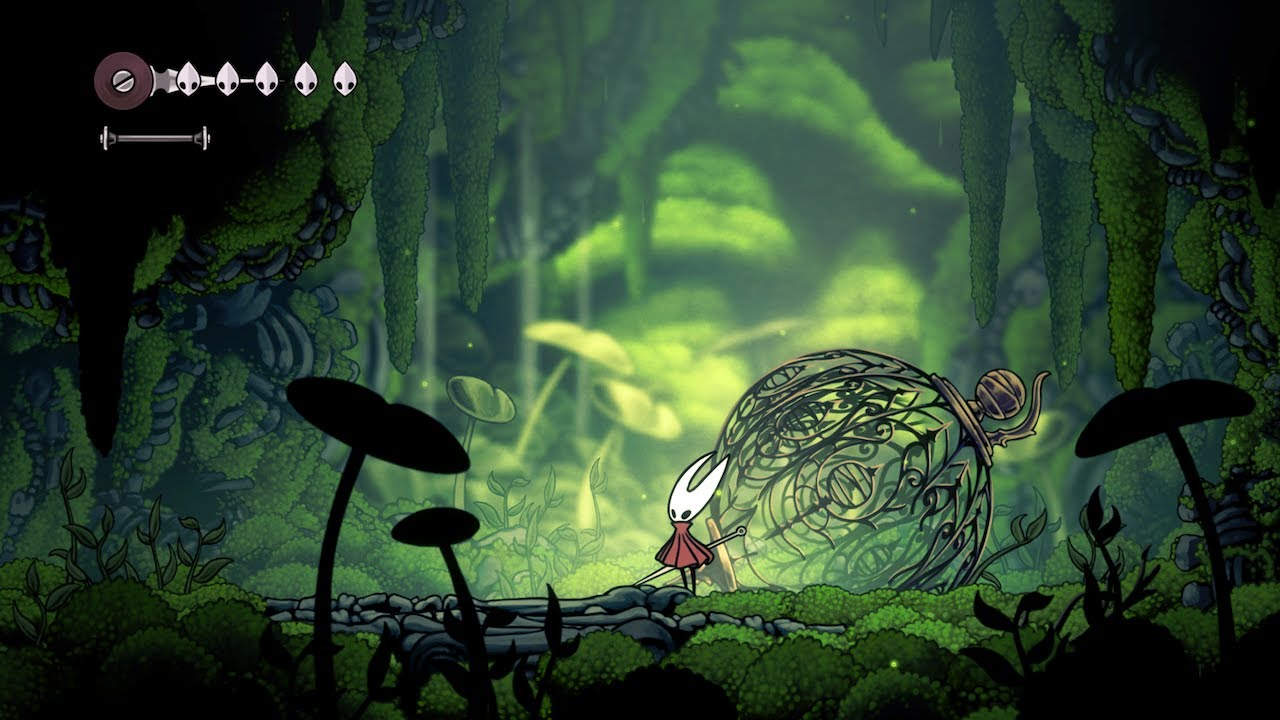
\includegraphics[width=0.8\textwidth]{images/figure1}
    \caption{Example figure 2}
    \label{fig:figure2}
\end{figure}
